\documentclass[9pt,dvipsnames]{beamer}
\usepackage{fontspec}
\usepackage{mathpazo}
\setsansfont{Bradley Hand ITC TT Bold}[
  BoldFont={*}, % Fallback to the same font for bold
  AutoFakeBold=2.5, % Simulate bold
  ItalicFont={*}, % Fallback to the same font for italic
  AutoFakeSlant=0.2 % Simulate italic
]

\setbeamerfont{section in toc}{family=\fontspec{Bradley Hand}, size=\normalsize}
\setbeamerfont{subsection in toc}{family=\fontspec{Bradley Hand}, size=\small}

% Since all text in Beamer is sans-serif by default, setting Bradley Hand as the sans font should apply it throughout the document
\setbeamerfont{structure}{family=\sffamily}
\setbeamerfont{normal text}{family=\sffamily}
\setbeamerfont{title}{family=\sffamily}
\setbeamerfont{frametitle}{family=\sffamily}
\setbeamerfont{itemize/enumerate body}{family=\sffamily}
\setbeamerfont{itemize/enumerate subbody}{family=\sffamily}

\AtBeginDocument{
  \usebeamerfont{normal text}
}
\usepackage{unicode-math} % For setting math font
\setmathfont{Libertinus Math} % Adjust the math font name as necessary

\usepackage{amsmath}
\usepackage[most]{tcolorbox}
\usepackage{graphicx}
\usepackage{bookmark}

%python 
\usepackage{listings}
% Default fixed font does not support bold face
\DeclareFixedFont{\ttb}{T1}{txtt}{bx}{n}{8} % for bold
\DeclareFixedFont{\ttm}{T1}{txtt}{m}{n}{8}  % for normal

% Custom colors
\usepackage{color}
\definecolor{deepblue}{rgb}{0,0,0.5}
\definecolor{deepred}{rgb}{0.6,0,0}
\definecolor{deepgreen}{rgb}{0,0.5,0}

\usepackage{listings}

% Python style for highlighting
\newcommand\pythonstyle{\lstset{
		language=Python,
		basicstyle=\ttm,
		morekeywords={self},              % Add keywords here
		keywordstyle=\ttb\color{deepblue},
		emph={MyClass,__init__},          % Custom highlighting
		emphstyle=\ttb\color{deepred},    % Custom highlighting style
		stringstyle=\color{deepgreen},
		frame=tb,                         % Any extra options here
		showstringspaces=false
}}


% Python environment
\lstnewenvironment{python}[1][]
{
	\pythonstyle
	\lstset{#1}
}
{}

% Python for external files
\newcommand\pythonexternal[2][]{{
		\pythonstyle
		\lstinputlisting[#1]{#2}}}

% Python for inline
\newcommand\pythoninline[1]{{\pythonstyle\lstinline!#1!}}

\usepackage{xcolor}  
\newcommand{\cb}[1]{{\color{CadetBlue}#1}}

\usepackage{pgfplots}
\pgfplotsset{compat=newest}
\setlength{\parskip}{0.5em}

\usepackage{setspace}
\setstretch{1.25}  
\usetheme{Singapore}
\setbeamertemplate{navigation symbols}{}

\setbeamertemplate{footline}{
    \leavevmode%
    \hbox{%
        \begin{beamercolorbox}[wd=.5\paperwidth,ht=2.25ex,dp=1ex,center]{author in head/foot}%
            % Customize this part if you want to add author or date information
        \end{beamercolorbox}%
        \begin{beamercolorbox}[wd=.5\paperwidth,ht=2.25ex,dp=1ex,right]{title in head/foot}%
            \usebeamerfont{title in head/foot}\insertframenumber{} / \inserttotalframenumber\hspace*{2ex} 
        \end{beamercolorbox}}%
    \vskip0pt%
}


% Custom Theorem Box Environment
\newenvironment{customtheorem}[1]
{%
	\tcolorbox[
	enhanced,
	colback=blue!5,
	colframe=blue!60!black,
	coltitle=black,
	colbacktitle=blue!5,
	fonttitle=\bfseries,
	attach boxed title to top left={yshift=-2mm, xshift=2mm},
	boxed title style={sharp corners},
	sharp corners,
	title=#1
	]
}
{%
	\endtcolorbox
}



\title{CSE574 Introduction to Machine Learning}
\subtitle{Adversarial Attack: An Overview}
\author{Jue Guo}
\institute{University at Buffalo}
\date{\today}

\begin{document}
\begin{frame}
    \titlepage
\end{frame}
\begin{frame}
    \frametitle{Outline}
    \tableofcontents
\end{frame}

\section{What are adversarial attacks?}
\begin{frame}
    \frametitle{Why?}
    \begin{itemize}
        \item Robustness = easiness to fail when input is perturbed. Perturbation can be in any kind. Robustness machine learning is a very rich topic.
        \item We will look at something very narrow, called \textbf{adversarial robusness}, also known as robustness against \textbf{attacks}.
        \item Adversairal attack is a very \textbf{hot} topic, as of today. We should not over-emphasize its importance. There are many other important problems.
    \end{itemize}
\end{frame}

\subsection{The surprising findings by Szegedy (2013) and Goodfellow (2014)}
\begin{frame}
    \frametitle{Adversarial Attack Example: FGSM}
    \begin{itemize}
        \item It is not difficult to fool a classifier
        \item The perturbation could be perceptually not noticeable
    \end{itemize}
    \begin{figure}[ht]
        \centering
        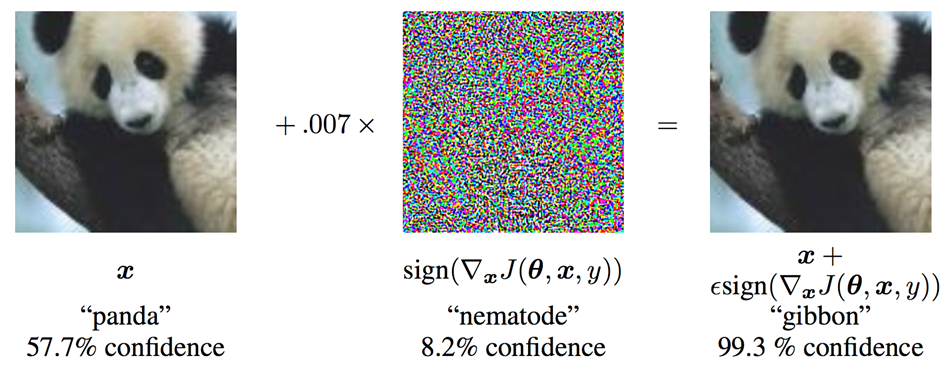
\includegraphics[width=0.8\textwidth]{imgs/adv_overview_1.png}
        \caption{Goodfellow et al. “Explaining and Harnessing Adversarial Examples”, https://arxiv.org/pdf/1412.6572.pdf}
    \end{figure}
\end{frame}

\begin{frame}
    \frametitle{Adversarial Attack Example: Szegedy’s 2013 Paper}

    \begin{itemize}
        \item This paper actually appears one year before Goodfellow's 2014 paper.
    \end{itemize}
    \begin{figure}[ht]
        \centering
        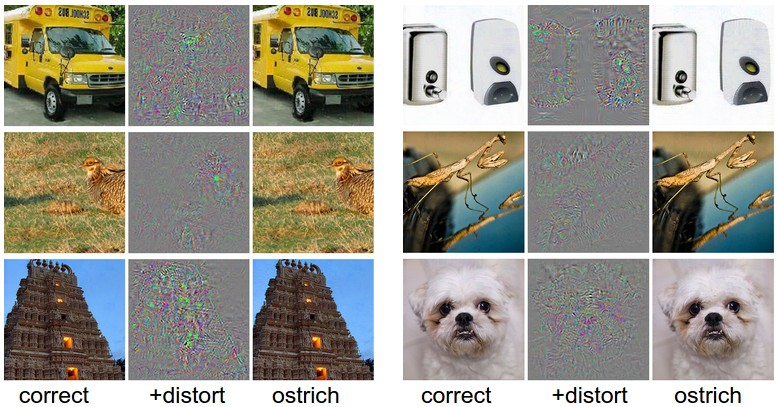
\includegraphics[width=0.8\textwidth]{imgs/adv_overview_2.png}
        \caption{Szegedy et al. Intriguing properties of neural networks https://arxiv.org/abs/1312.6199}
    \end{figure}
\end{frame}

\subsection{Example of attacks}
\begin{frame}
    \frametitle{Adversarial Attack: Targeted Attack}
    \begin{itemize}
        \item Targeted Attack
    \end{itemize}
    \begin{figure}[ht]
        \centering
        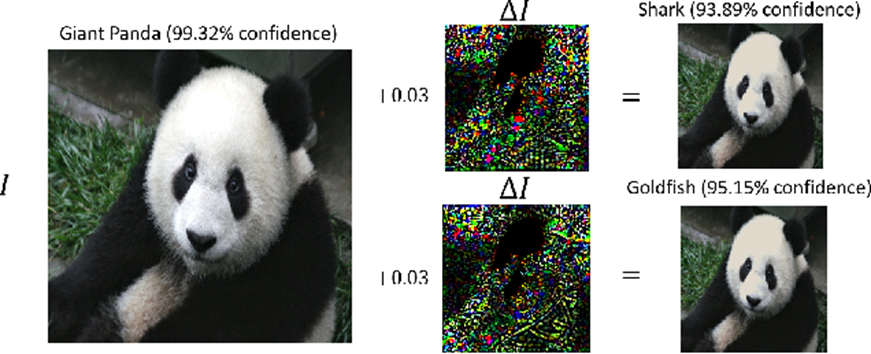
\includegraphics[width=0.8\textwidth]{imgs/adv_overview_3.png}
        \caption{Adversarial Examples Detection in Deep Networks with Convolutional Filter Statistics, https://arxiv.org/abs/1612.07767}
    \end{figure}
\end{frame}

\begin{frame}
    \frametitle{Adversarial Attack Example: One Pixel}
    \begin{itemize}
        \item One-pixel Attack
    \end{itemize}
    \begin{figure}
    	\centering
    	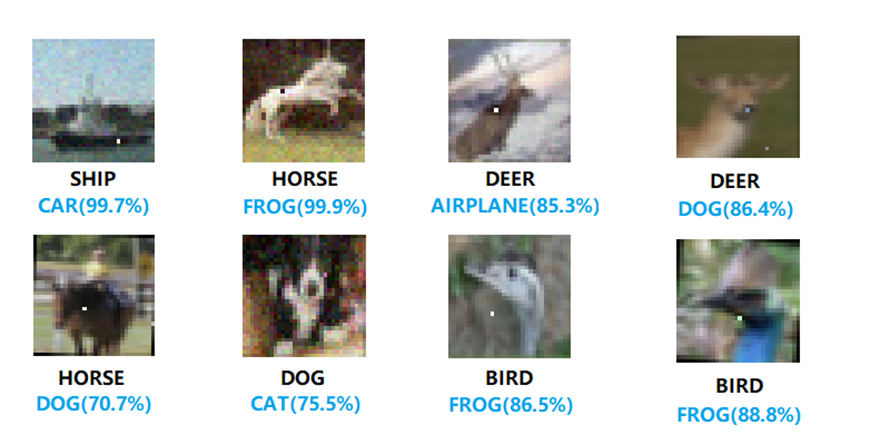
\includegraphics[width=0.8\textwidth]{imgs/adv_overview_4.png}
    	\caption{One pixel attack for fooling deep neural networks https://arxiv.org/abs/1710.08864}
    \end{figure}
\end{frame}
\begin{frame}
	\frametitle{Adversarial Attack Example: Patch}
	\begin{itemize}
		\item Adding a patch
	\end{itemize}
	    \begin{figure}
		\centering
		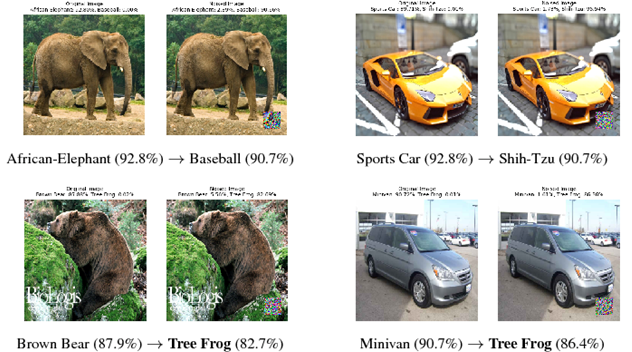
\includegraphics[width=0.8\textwidth]{imgs/adv_overview_5.png}
		\caption{LaVAN: Localized and Visible Adversarial Noise, https://arxiv.org/abs/1801.02608}
	\end{figure}
\end{frame}

\subsection{Physical Attacks}
\begin{frame}
	\frametitle{Adversarial Attack Example: Stop Sign}
	\begin{itemize}
		\item The Michigan / Berkely Stop Sign
	\end{itemize}
	\begin{figure}[htbp]
		\centering
		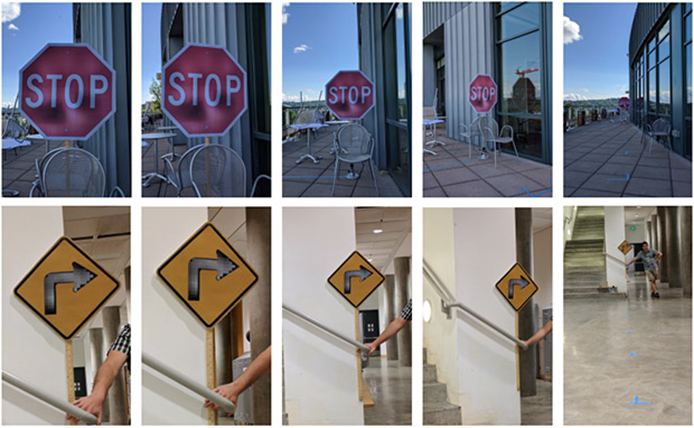
\includegraphics[width=0.8\textwidth]{imgs/adv_overview_6.png}
		\caption{Robust Physical-World Attacks on Deep Learning Models https://arxiv.org/abs/1707.08945}
	\end{figure}
\end{frame}

\begin{frame}
	\frametitle{Adversarial Attack Example: Turtle}
	\begin{itemize}
		\item The MIT 3D Turtle
	\end{itemize}
	\begin{figure}[htbp]
		\centering
		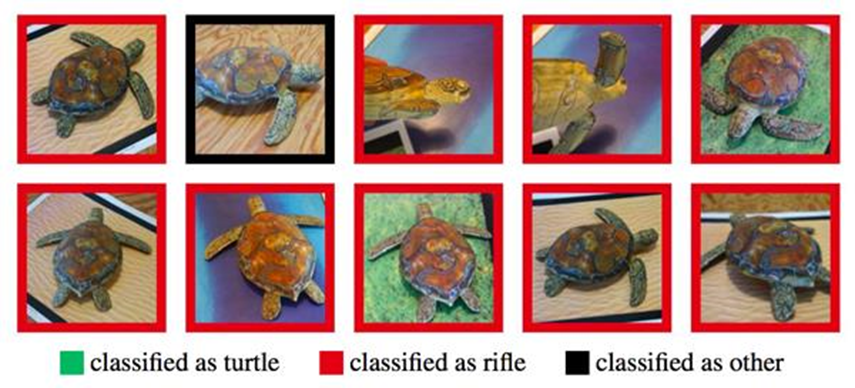
\includegraphics[width=0.8\textwidth]{imgs/adv_overview_7.png}
		\caption{Synthesizing Robust Adversarial Examples https://arxiv.org/pdf/1707.07397.pdf https://www.youtube.com/watch?v=YXy6oX1iNoA}
	\end{figure}
	
\end{frame}

\begin{frame}
	\frametitle{Adversarial Attack Example: Glass}
	\begin{itemize}
		\item CMU Glass
	\end{itemize}
	\begin{figure}[htbp]
		\centering
		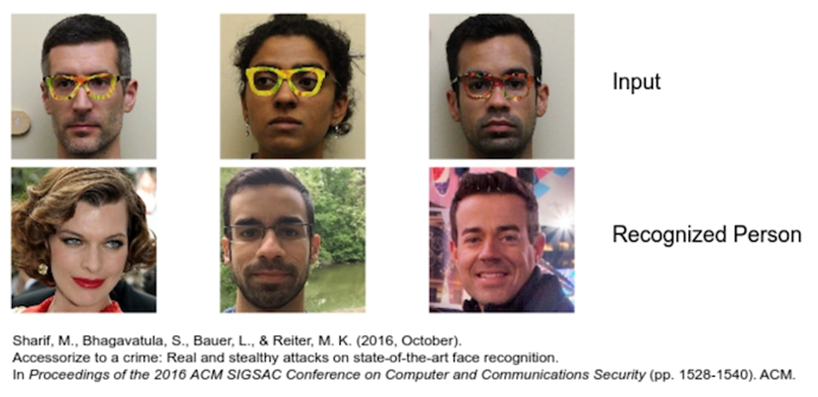
\includegraphics[width=0.8\textwidth]{imgs/adv_overview_8.png}
		\caption{Accessorize to a Crime: Real and Stealthy Attacks on State-of-the-Art Face Recognition 
			https://www.cs.cmu.edu/ \sim sbhagava/papers/face-rec-ccs16.pdf https://www.archive.ece.cmu.edu/ \sim lbauer/proj/advml.php}
	\end{figure}
\end{frame}

\section{Basic Terminologies}
\begin{frame}
	\frametitle{Definition: Additive Adversarial Attack}
	\begin{customtheorem}{Additive Adversarial Attack}
Let \(x_{0} \in \mathbb{R}^{d}\) be a data point belong to class \(\mathcal{C}_{i}\). Define a target class \(\mathcal{C}_{t}\)
An additive adversarial attack is an addition of a perturbation \(r \in \mathbb{R}^{d}\)
such that the perturbed data
$$
x=x_{0}+\boldsymbol{r}
$$
is misclassified as \(\mathcal{C}_{t}\).
	\end{customtheorem}
	\begin{figure}[htbp]
		\centering
		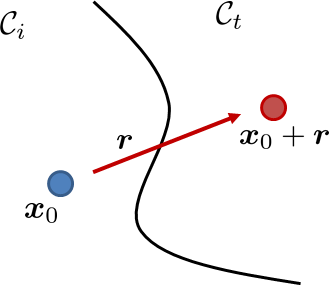
\includegraphics[width=0.2\textwidth]{imgs/adv_overview_9.png}
	\end{figure}
\end{frame}

\begin{frame}
	\frametitle{Definition: General Adversarial Attack}
	\begin{customtheorem}{General Adversarial Attack}
		Let \(x_{0} \in \mathbb{R}^{d}\) be a data point belong to class \(\mathcal{C}_{i}\). Define a target class \(\mathcal{C}_{t}\)
		An adversarial attack is a mapping \(\mathcal{A}: \mathbb{R}^{d} \rightarrow \mathbb{R}^{d}\) such that the
		perturbed data
		$$
		x=\mathcal{A}\left(x_{0}\right)
		$$
		is misclassified as \(\mathcal{C}_{t}\).
	\end{customtheorem}
		\begin{figure}[htbp]
		\centering
		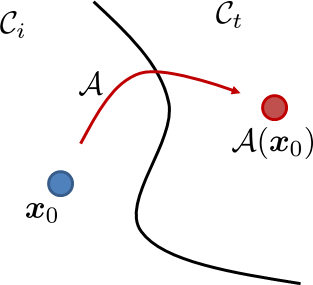
\includegraphics[width=0.2\textwidth]{imgs/adv_overview_10.png}
	\end{figure}
\end{frame}

\section{Multi-class Problem}
\begin{frame}
	\frametitle{Multi-class Problem}
	\textbf{Approach 1: One-on-One}
			\begin{figure}[htbp]
		\centering
		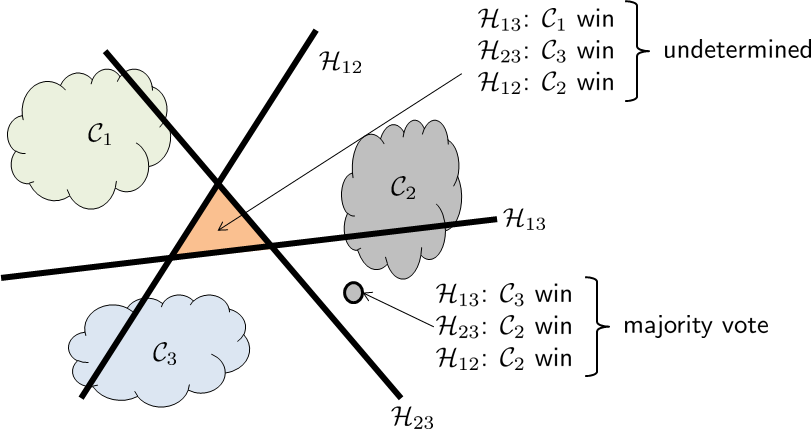
\includegraphics[width=0.5\textwidth]{imgs/adv_overview_11.png}
	\end{figure}
	\begin{itemize}
		\item Class $i$ vs. Class $j$
		\item Give me a point, check which class has more votes
		\item There is an undetermined region
	\end{itemize}
\end{frame}

\begin{frame}
	\frametitle{The Multi-Class Problem}
	\textbf{Approach 2: One-on-All}
	\begin{figure}[htbp]
		\centering
		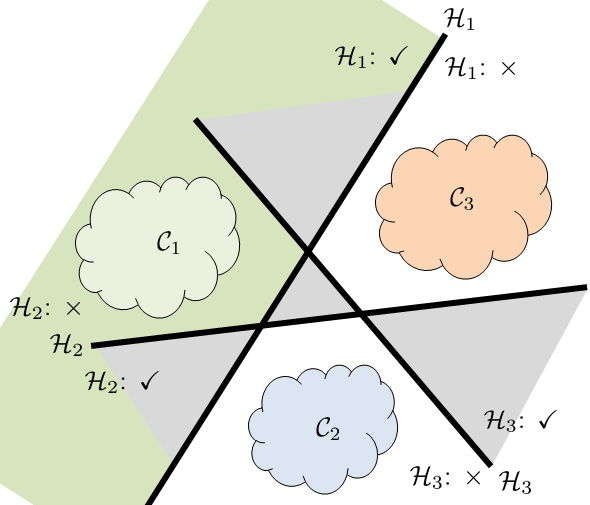
\includegraphics[width=0.4\textwidth]{imgs/adv_overview_12.png}
	\end{figure}
	\begin{itemize}
		\item Class $i$ not Class $i$
		\item Give me a point, check which class has no conflict
		\item There are undetermined regions
	\end{itemize}
\end{frame}

\begin{frame}
	\frametitle{The Multi-Class Problem}
	\textbf{Approach 3: Linear Machine}
		\begin{figure}[htbp]
		\centering
		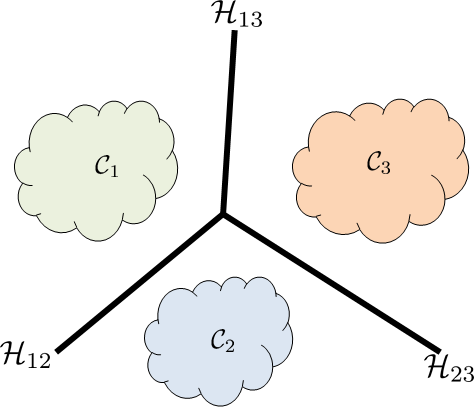
\includegraphics[width=0.4\textwidth]{imgs/adv_overview_13.png}
	\end{figure}
	\begin{itemize}
		\item Every point in the space gets assigned a class. 
		\item You give me \(x\), I compute \(g_{1}(x), g_{2}(x), \ldots, g_{K}(x)\)
		\item If \(g_{i}(\boldsymbol{x}) \geq g_{j}(\boldsymbol{x})\) for all \(j \neq i\), then \(\boldsymbol{x}\) belongs to class \(i\)
	\end{itemize}
\end{frame}
\end{document}